Earthquakes are unpredictable phenomena, which damaging capabilities can be catastrophic. Given the limited nature of resources, its correct allocation is vital to mitigate the damage in the aftermath. Technology makes the labors of logistics and rescues a lot easier. This chapter explores the motivation, history, objective and scope of the present work.\\

\section{Motivation}

Massive collaboration proved to be a fundamental resource to face the aftermath caused by the earthquake of September 19, 2017, in Mexico City. The use of social networks allowed communication between rescue, logistics, and civil society. We learned lessons about the scope and limitations of this association.\\

However, what happens when the conditions and technological infrastructure of large cities do not exist? This work explores other possibilities in which current technologies can help us when the situation in which the natural disaster occurs is different. Focusing on the study of images captured by drones during the days after the earthquake of September 7, 2017, in towns of the state of Oaxaca, we propose an analytical framework that allows detecting damaged areas in an automated way.\\

To do this, we applied techniques that allow the use of models that have been previously trained in massive supercomputers, adjusting them to our particular problem. This process reduces the number of resources needed, in both time and infrastructure, to obtain results with high accuracy. In the future, this will allow allocating efforts in a more agile and efficient manner.\\

\section{History}

Given to the particular geographical conditions, Mexico is very prone to seismic activity. The Cocos and the Rivera plates subduct below the North American plate, and the Pacific plate separates from the North American plate along the Baja California Gulf \cite{AG3315}.\\

\begin{figure}[h]
  \begin{center}
    \subfigure{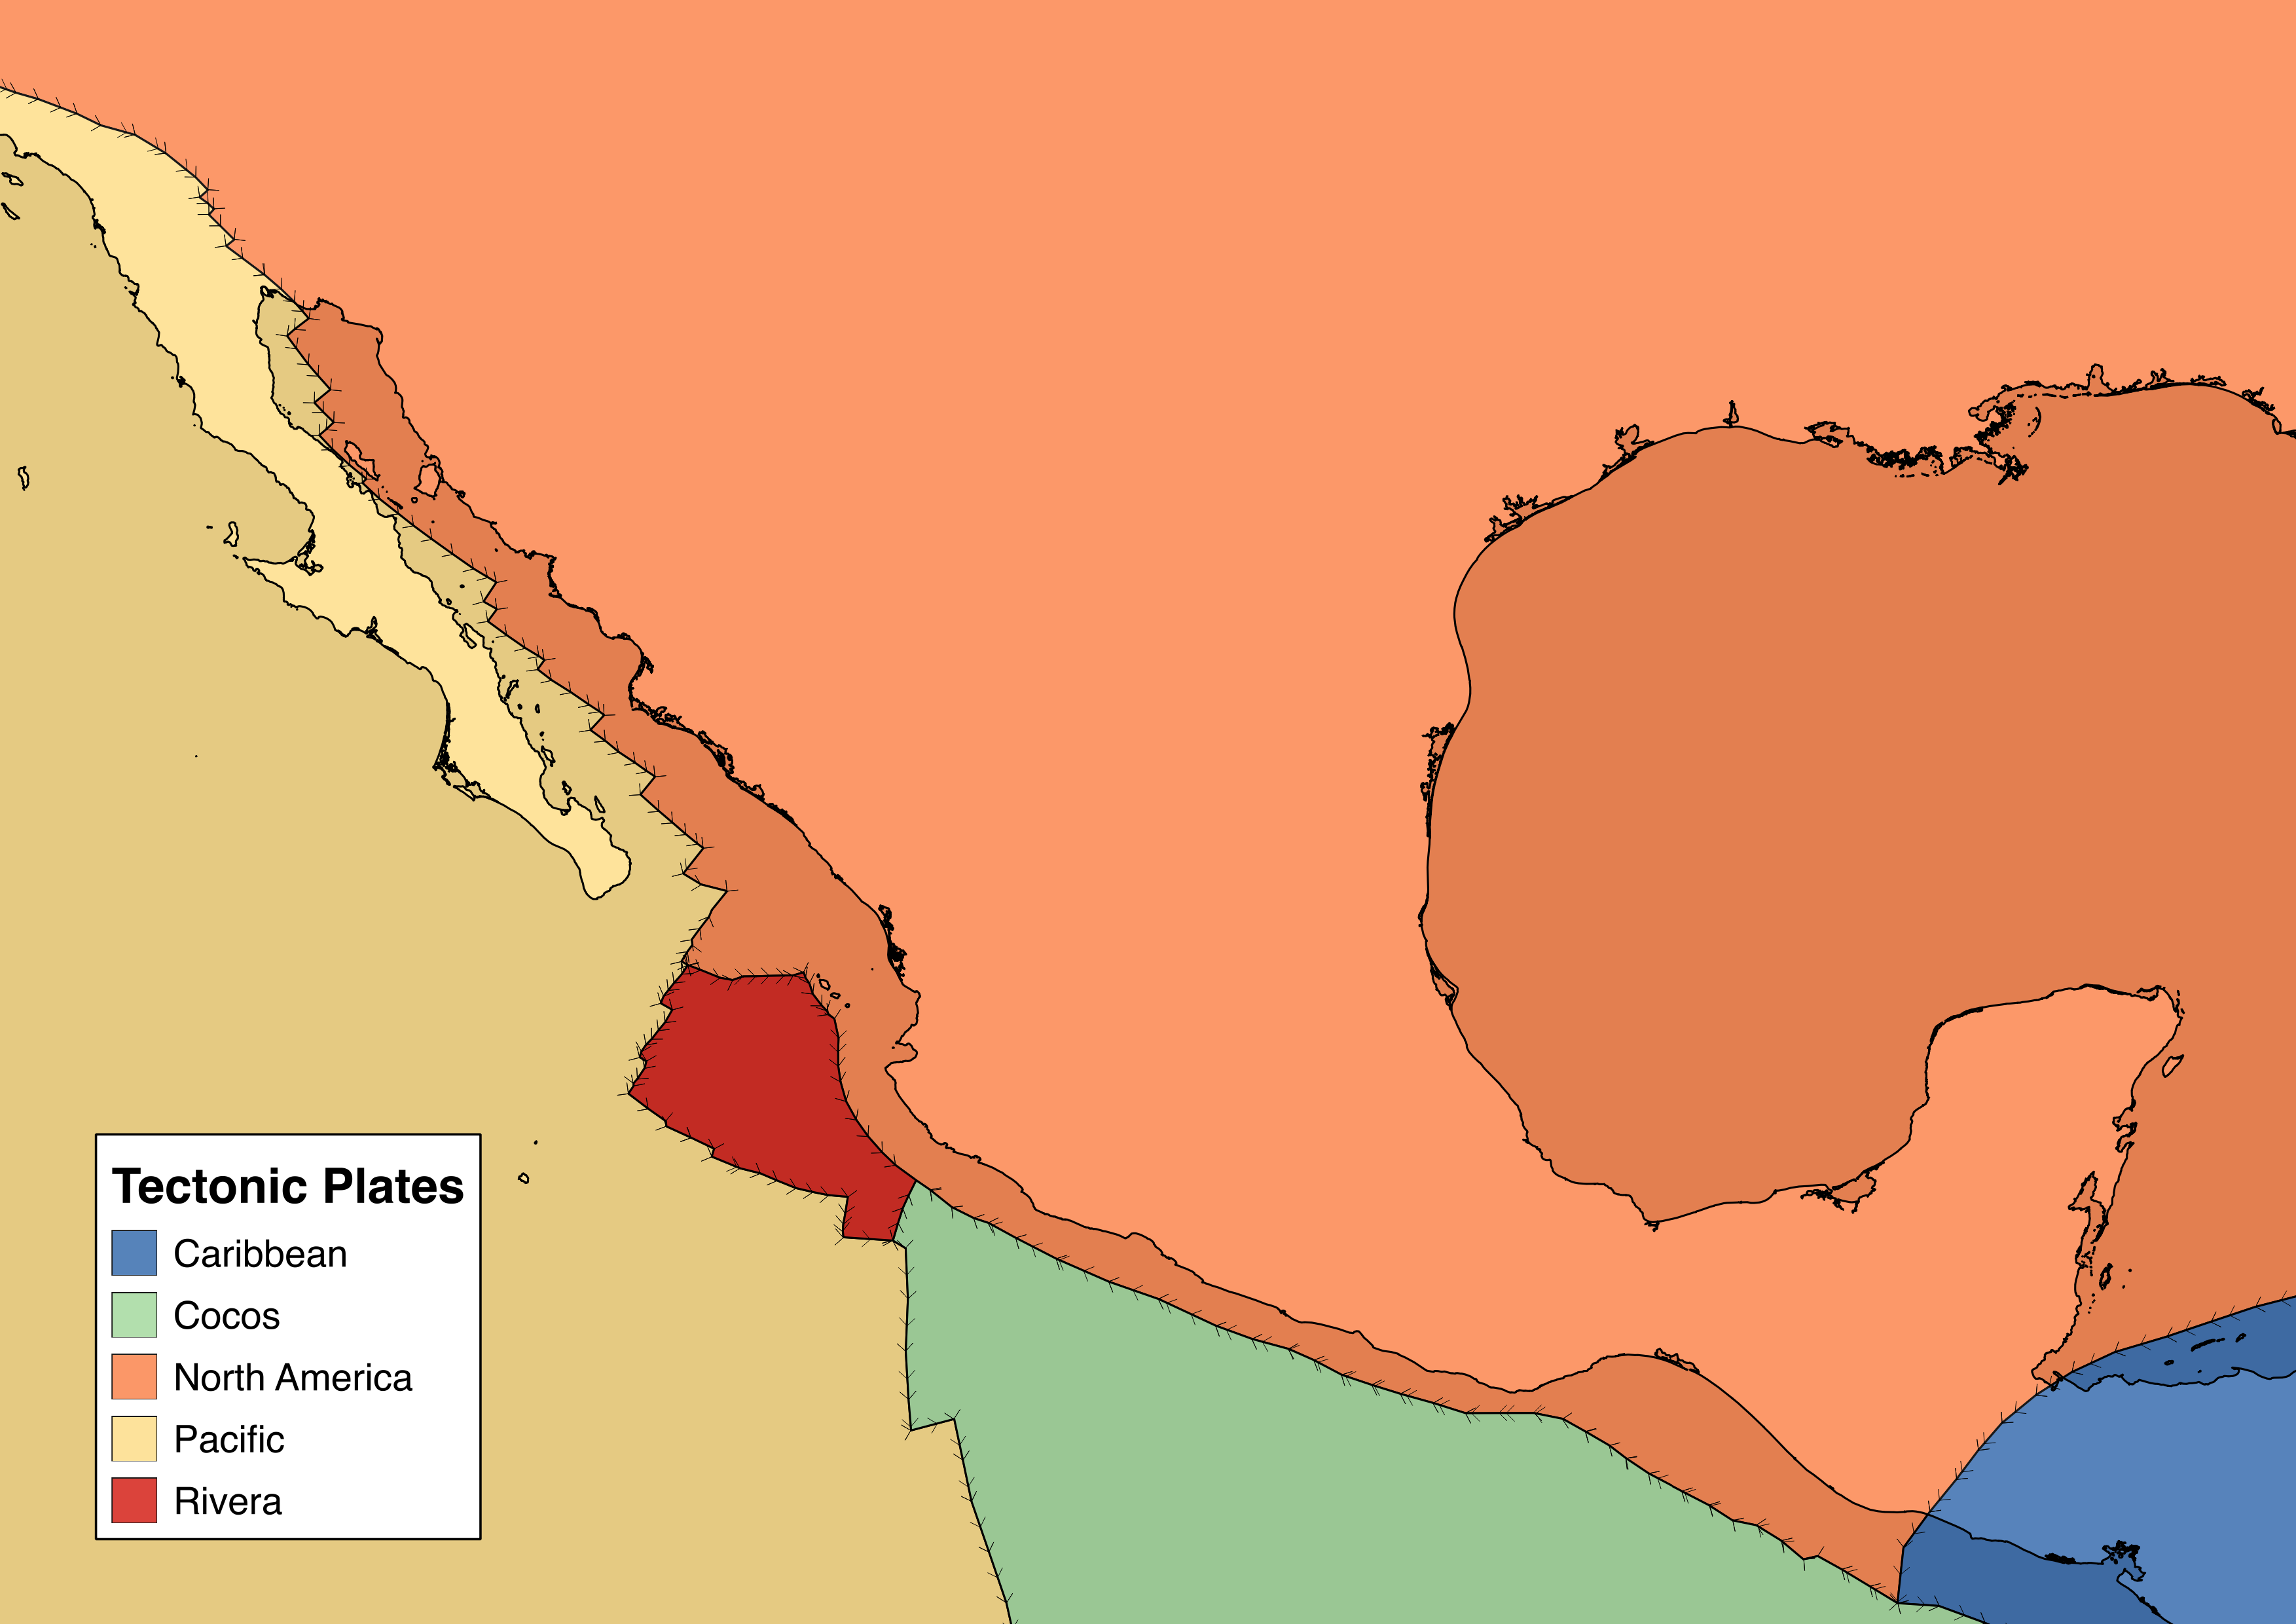
\includegraphics[width=1\textwidth]{images/plates.png}}
  \end{center}
  \label{fig:plates}
  \caption{We can see the five tectonic plates meeting near Mexico.}
\end{figure}

According to historical research, there has been a registry of these natural disasters since the Pre-Columbian age. The level of material damage and the death toll has been increasing ever since as the population and the cities grew. In figure \cite{fig:codice} we can see a pictogram that according to \cite{sismosmexico} means "in the year 11 rabbit the earth trembled during the night".\\


\begin{figure}[h]
  \begin{center}
    \subfigure{\label{fig:codice}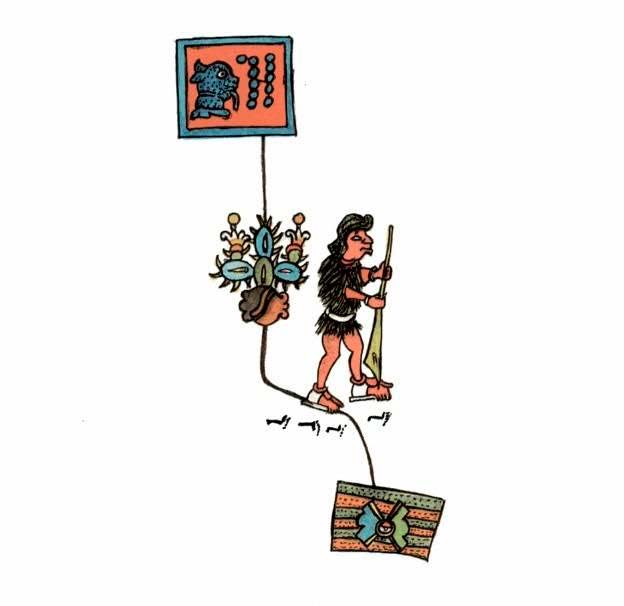
\includegraphics[width=1\textwidth]{images/codice.jpg}}
  \end{center}
  \caption{Pictogram depicting an earthquake.}
\end{figure}

The use of cartography to place the damage information also is useful not only to allocate resources in the aftermath of the disaster but also serves as historical evidence. In figure \cite{fig:quake1800} taken from \cite{AG3316} we can see the buildings damaged by an earthquake known as the *San Juan de Dios* earthquake \footnote{Back then the earthquakes where name accordingly to the day in which they happened.}. This event dates back to March 8, 1800, years before the Mexican Independence, during an age of economic and social prosperity.\\

According to historical records, a critical earthquake occurred in the year 1787, causing a massive tsunami that affected the coasts of Oaxaca along 450 kilometers. Paradoxically, this catastrophic event didn't produce as much damage as recent ones due to the lack of established cities in the state back then.\\

Years 1845 and 1858 also had significant earthquake events that destroyed infrastructure in Mexico city. We can find a mapping of the damaged buildings in \cite{AG3316}. The fall of the iconic Angel of Independence was the result of an earthquake on July 28, 1957, in an event that left dozens of deaths.\\

Nevertheless, the real breaking point in the Mexican seismological history came on September 19, 1985. That morning, an 8.1 magnitude earthquake stroke the city collapsing many buildings and leaving a death toll measured by thousands. Next day, the aftershock collapsed even more buildings, damaged the day before. The destruction and chaos that the earthquake provoked still lingers in the memory of the people that witnessed such a terrifying event.\\

The way people reacted after September 19, 2017, was because they grew up in an ambient of constant fear to the quakes.\\

Two earthquakes took place during September 2017. While the second one devastated Mexico City, attracting help from all over the world, the first one was less known even though it was the earthquake with the highest magnitude that has hit the country in the last century. Both were catastrophic for the state of Oaxaca. The locality of Juchitan de Zaragoza was one of the most affected, buildings collapsed, and several people died.\\

\begin{figure}[h]
  \begin{center}
    \subfigure{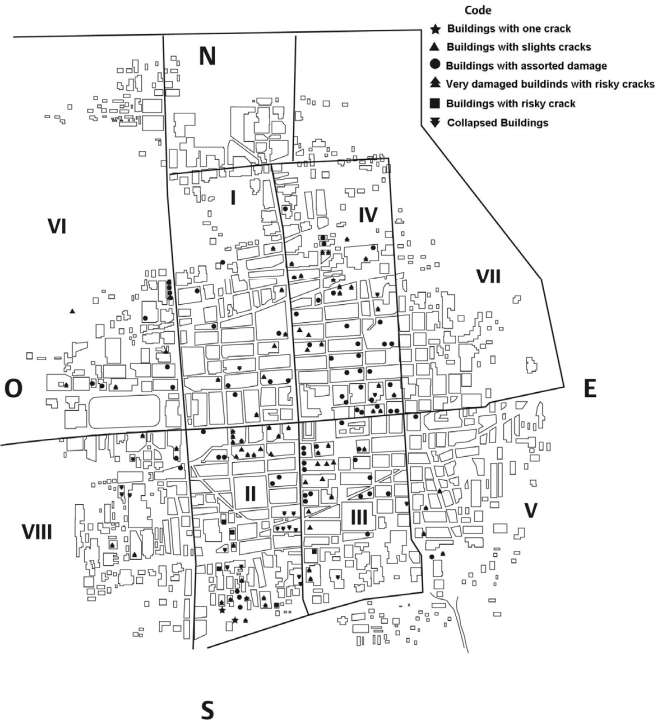
\includegraphics[width=1\textwidth]{images/quake1800.png}}
  \end{center}
  \label{fig:quake1800}
  \caption{A damaged building map for the *San Juan de Dios* earthquake in Mexico City.}
\end{figure}


\section{Objective}

It is not coincidental that our brief historical summary focused mainly in Mexico City. The lack of infrastructure and the distance from large cities make it harder to reach certain towns with resources and aid. We want to explore the use of new technologies to focus our efforts and use them better.\\

The National Center for Prevention of Disasters (CENAPRED) provided us with imagery taken on the days after the Chiapas earthquake took place. They flew drones over the towns of Juchitan de Zaragoza, Santa Maria Xadani, and Union Hidalgo. We propose to use those images to train a model that lets us geolocate collapsed buildings and create a map with them. In the case of another catastrophic event of similar nature, drones can be sent to fly over the affected area, and our proposed tool can be used to narrow dramatically the places which assessment teams must visit. This would reduce the amount of resources and time needed to correctly asses the damage in the earthquake aftemath.\\

In Mexico, CENAPRED is in charge of channeling financial resources in the case of a natural disaster.\\

We want to explore the use of Convolutional Neural Networks (CNNs) in this context. We believe that this field is useful for disaster assessment, and will bloom in the coming years.\\

\section{Scope}

We don't pretend to provide a perfect mapping of every single collapsed building. We understand the inherent limitations of automatic methods, but we believe that we can achieve greater things working together with this new tools. Machine learning methods are not a panacea by no means, but a useful device that can help us reach places we could just imagine before.\\

We have to keep in mind that this is only the beginning and that there is vast room for improvement. The literature review in which we will dive more in-depth in the next chapter suggests ways of improving the results that we got, but its implementation is out of the scope of this work.\\

It would be far too ambitious to cover every topic that is involved in the process of the classification using CNNs. We want to explain how do the networks work to a certain extent, but it is not in the scope of this work to untangle every single detail.\\

As we already mentioned, the field of Computer Vision is in its climax. Reviewing every single article written on the topic would be a daunting task. We offer a brief literature review that gives some context about the state-of-the-art, and we hope to build upon ideas and efforts done by a myriad of people. We aimed to create a system capable of processing imagery and that allows an institution such as CENAPRED to deploy it into a cluster for efficient computation.\\